\chapter{Meltdown e il sistema di protezione KAISER}
La sicurezza dei sistemi informatici attuali si fonda sull'isolamento della memoria,
ad esempio marcando come privilegiati gli indirizzi di memoria kernel e bloccando eventuali
accessi da parte di programmi utente \cite{lettieri:protezione}. 
\textbf{Meltdown} è un tipo di attacco informatico che sfrutta un effetto
collaterale dell'esecuzione fuori ordine nei processori moderni per leggere locazioni di memoria scelte in maniera
arbitraria. L'attacco funziona su varie microarchitetture Intel prodotte sin dal 2010, indipendentemente dal sistema
operativo in uso. Meltdown è quindi in grado di accedere arbitrariamente a qualsiasi locazione di memoria protetta
(afferenti al kernel o ad altri processi) senza necessitare alcun permesso o privilegio da parte del
sistema \cite{lipp:meltdown}.

Meltdown rompe quindi tutti i meccanismi di sicurezza che si basano sull'isolamento degli spazi di indirizzamento, andando a colpire milioni di utenti. Il sistema di protezione KAISER, sviluppato originariamente per KASLR \cite{gruss:kaslr}, ha l'importante effetto secondario di impedire l'utilizzo di Meltdown \cite{lipp:meltdown}.


\section{Background}

\subsection{Esecuzione Fuori Ordine}
\label{sec:esecuzione-fuori-ordine}

\subsection{Spazi di indirizzamento}
\label{sec:spazi-di-indirizzamento}
\begin{figure}
	\centering
	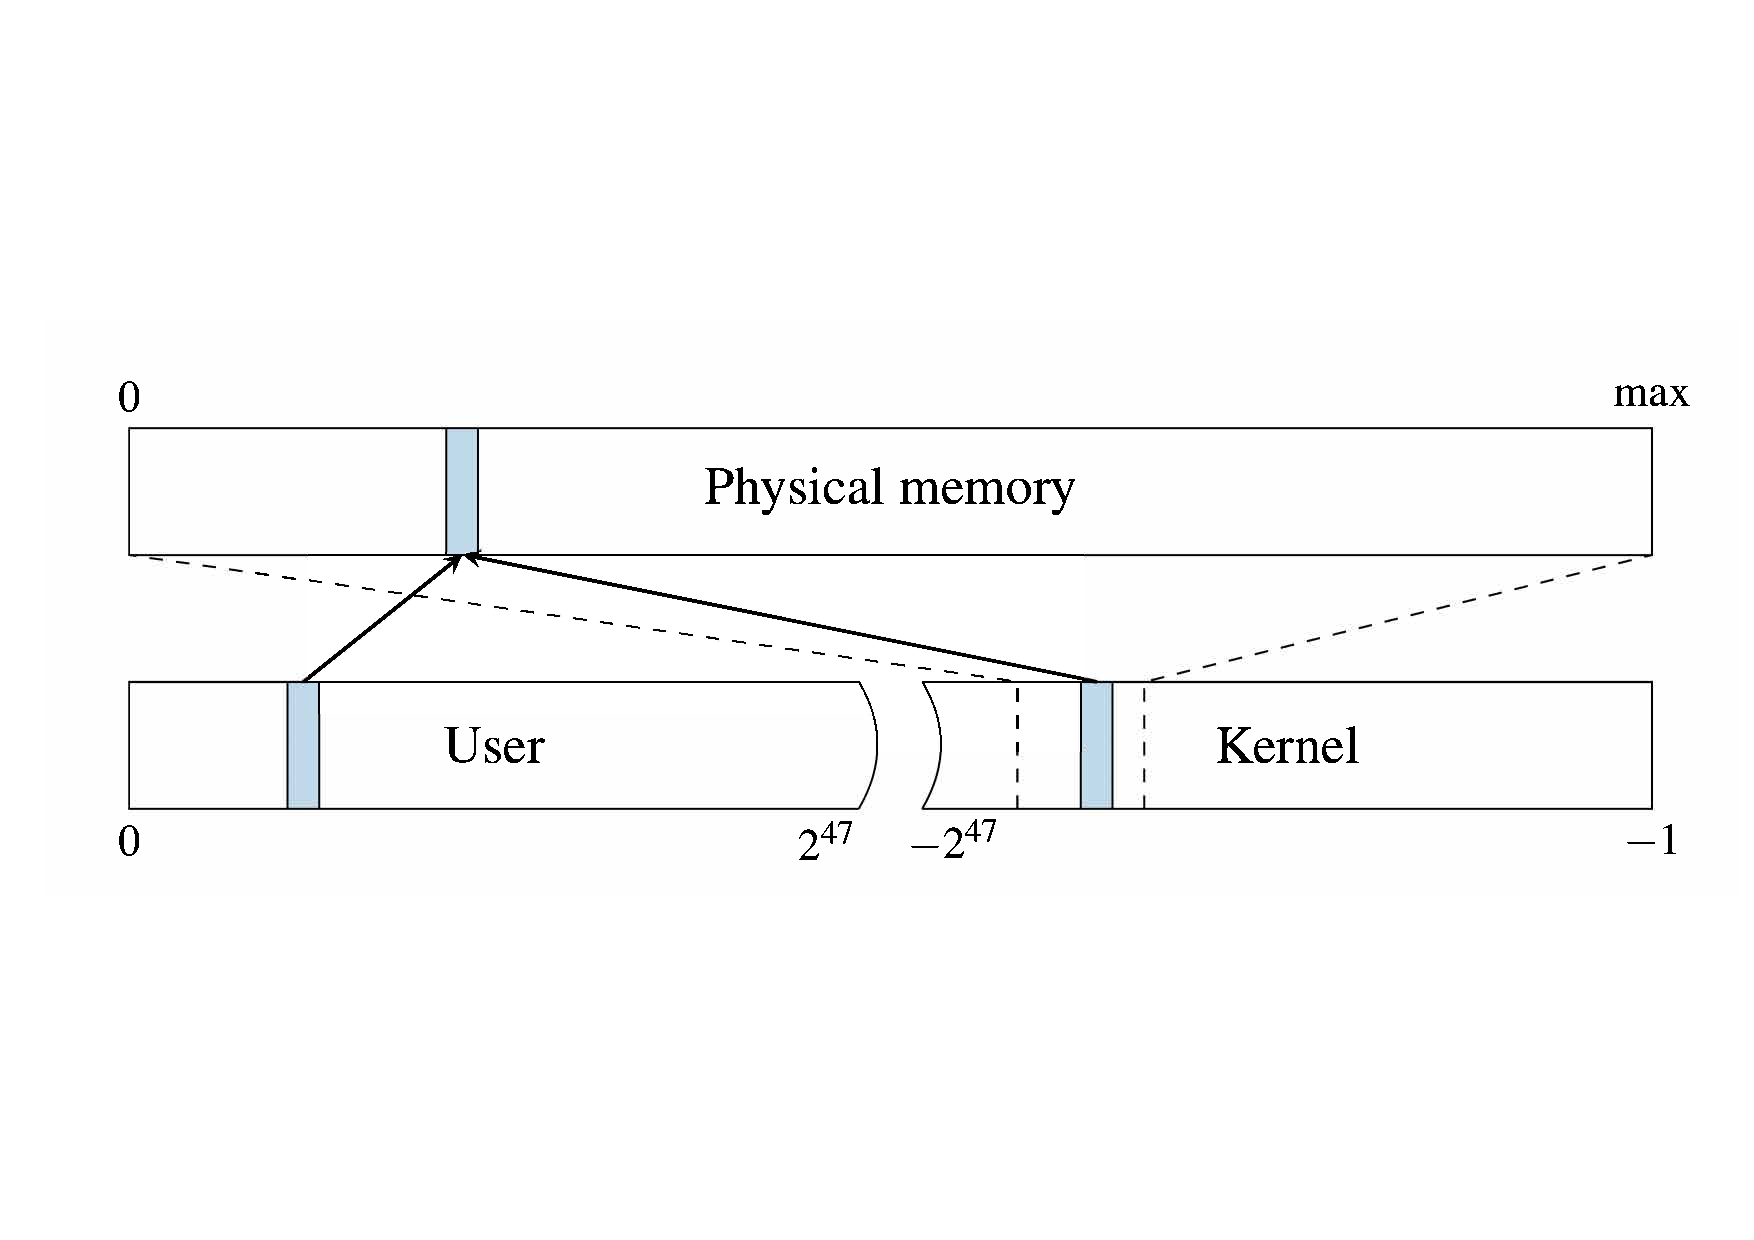
\includegraphics[width=0.5\textwidth]{"img/memoria-fisica.pdf"}
	\caption{text} % TODO
	\label{fig:memoria-fisica}
\end{figure}

Per risolvere diversi problemi, in particolare l'isolamento dei processi \cite{lettieri:paginazione}, le CPU supportano l'utilizzo di spazi d'indirizzamento virtuali, in cui gli indirizzi virtuali (relativi al singolo processo) vengono tradotti in indirizzi fisici. 
Lo spazio d'indirizzamento di un processo (ovvero tutti i possibili indirizzi che un processo può generare) viene suddiviso in regioni dette \emph{pagine} che possono essere mappate individualmente nella memoria fisica attraverso una tabella di traduzione multivello. 
Ogni processo possiede una propria tabella di traduzione che traduce tutti e soli i suoi indirizzi virtuali e che definisce le proprietà di protezione delle varie zone di memoria. 

Ogni processo può quindi riferirsi esclusivamente agli indirizzi appartenenti al proprio spazio di indirizzamento virtuale. Per permettere l'utilizzo 


\subsection{Attacchi Cache}
Al fine di velocizzare gli accessi alla RAM, le CPU contengono buffer di memoria molto veloce ma di dimensioni limitate che costituiscono la cosiddetta \emph{memoria cache}. La memoria cache maschera i tempi di latenza estremamente lunghi per l'accesso alla memoria centrale (molto lenta in confronto alla cache) conservando le locazioni di memoria che, secondo principi statistici come la \emph{località spaziale} (se un programma accede ad un certo indirizzo, è molto probabile che in breve tempo accederà ad un indirizzo vicino)  e la \emph{località temporale} (se un programma accede ad un certo indirizzo, è molto probabile che in breve tempo vi accederà di nuovo), è più probabile vengano indirizzate dalla CPU nel breve periodo \cite{lettieri:cache}.

Gli attacchi a canale laterale (\emph{side-channel attacks}) contro la cache sfruttano questa differenza di tempo di accesso introdotta dalla cache stessa. Negli attacchi Flush+Reload \cite{yaron:flush-reload}, usati da Meltdown \cite{lipp:meltdown}, l'attaccante è in grado di determinare se una locazione di memoria è stata precedentemente caricata in cache, misurando il tempo impiegato da un'operazione di lettura.

%%
\section{Come agisce Meltdown}
L'attacco Meltdown consiste in tre passi fondamentali \cite{lipp:meltdown}:
\begin{enumerate}
	\item Leggere il contenuto di una locazione di memoria inaccessibile dall'attaccante, causando il lancio di un'eccezione di protezione
	\item Accedere in maniera speculativa ad una linea di memoria cache in base al contenuto segreto della locazione protetta
	\item Usare un'attacco di tipo Flush+Reload per determinare il contenuto segreto in base a quale linea di memoria è stata acceduta
\end{enumerate}

\subsection{Passo 1: Leggere del segreto}
Nel prima passo di Meltdown, l'attaccante cerca di accedere ad una zona di memoria protetta, ad esempio la memoria kernel.
Il tentativo di accesso ad una pagina non accessibile da livello utente fa in modo che la CPU sollevi un'eccezione di protezione, che generalmente termina il processo. 
Tuttavia, a causa dell'esecuzione fuori ordine, la CPU potrebbe aver già eseguito l'istruzione di accesso in maniera speculativa \emph{prima} delle istruzioni relative all'eccezione di protezione, al fine di minimizzare i tempi di latenza (vedi paragrafo \ref{sec:esecuzione-fuori-ordine}).
In questo modo la CPU accederebbe in maniera speculativa alla locazione di memoria desiderata prima che il processo venga terminato.

Grazie al lancio dell'eccezione, le eventuali istruzioni eseguite in maniera speculativa, che non sarebbero docute essere eseguite in quanto relative ad una previsione di salto \emph{errata}, non vengono \emph{ritirate} dalla CPU e non hanno così alcun effetto sulla macroarchitettura in generale (memoria centrale e registri logici non speculativi del processore) \cite{frosini:calcolatori2}.

\subsection{Passo 2: Trasmettere il segreto}
Per poter trasmettere il segreto, si utilizza un \emph{probe array}, di dimensione pari a 256 pagine virtuali e allocato precedentemente nella memoria del processo attaccante, assicurandosi che \emph{nessuna porzione dell'array sia presente nella cache}. 
La sequenza di transient instruction contiene un accesso ad un elemento del probe array, il cui offset è calcolato moltiplicando il valore del byte per la dimensione di una pagina virtuale (tipicamente e nel nostro sistema  è \emph{4KB}~\cite{lettieri:paginazione}).

Quando la CPU gestisce l'eccezione di protezione causata dal Meltdown, le transient instruction non vengono ritirate dalla CPU, senza avere dunque effetti a livello di macroarchitettura. Sebbene quindi non sia possibile rendere direttamente disponibile il segreto dal programma utente, si hanno importanti effetti secondari a livello di microarchitettura, in particolare nella memoria cache~\cite{lipp:meltdown}.

Durante l'esecuzione speculativa, infatti, la locazione di memoria all'interno del probe array che viene acceduta dalla CPU, viene memorizzata in memoria cache e vi rimane anche in seguito all'annullamento degli effetti delle transient instruction, rendendola vulnerabile ad un attacco side-channel.

L'utilizzo del valore segreto moltiplicato per la dimensione della pagina, ci garantisce sia una precisa \emph{correlazione} tra il valore segreto e la locazione caricata in memoria, sia che a differenti valori della locazione di memoria saranno accedute differenti \emph{pagine} del probe array.
Ciò previene il fatto che il prefetcher hardware (per ragioni di ottimizzazione) potrebbe caricare in cache anche le locazioni di memoria adiacenti a quella acceduta, rendendo impossibile determinare quale locazione di memoria sarebbe stata indirizzata se non fosse stato utilizzato a priori questo accorgimento.

\subsection{Passo 3: Ricevere del segreto}

Dopo che la sequenza di istruzioni del passo 2 è stata eseguita, in cache è presente esattamente una linea di memoria del probe array.
L'offset di questa linea è dipendente esclusivamente dal valore segreto presente nell'arbitaria locazione di memoria protetta.
Grazie a ciò, l'attaccante può effettuare un'attacco Flush+Reload~\cite{yaron:flush-reload}, iterando attraverso le 256 pagine del probe array e misurando il tempo di accesso per il primo elemento di ogni pagina (vedi figura \vref{fig:probe-array}).
In base a quanto detto finora, la pagina con la latenza minore è l'unica presente in memoria cache e il numero della pagina è il valore segreto letto dalla memoria protetta.

\begin{figure}
	\centering
	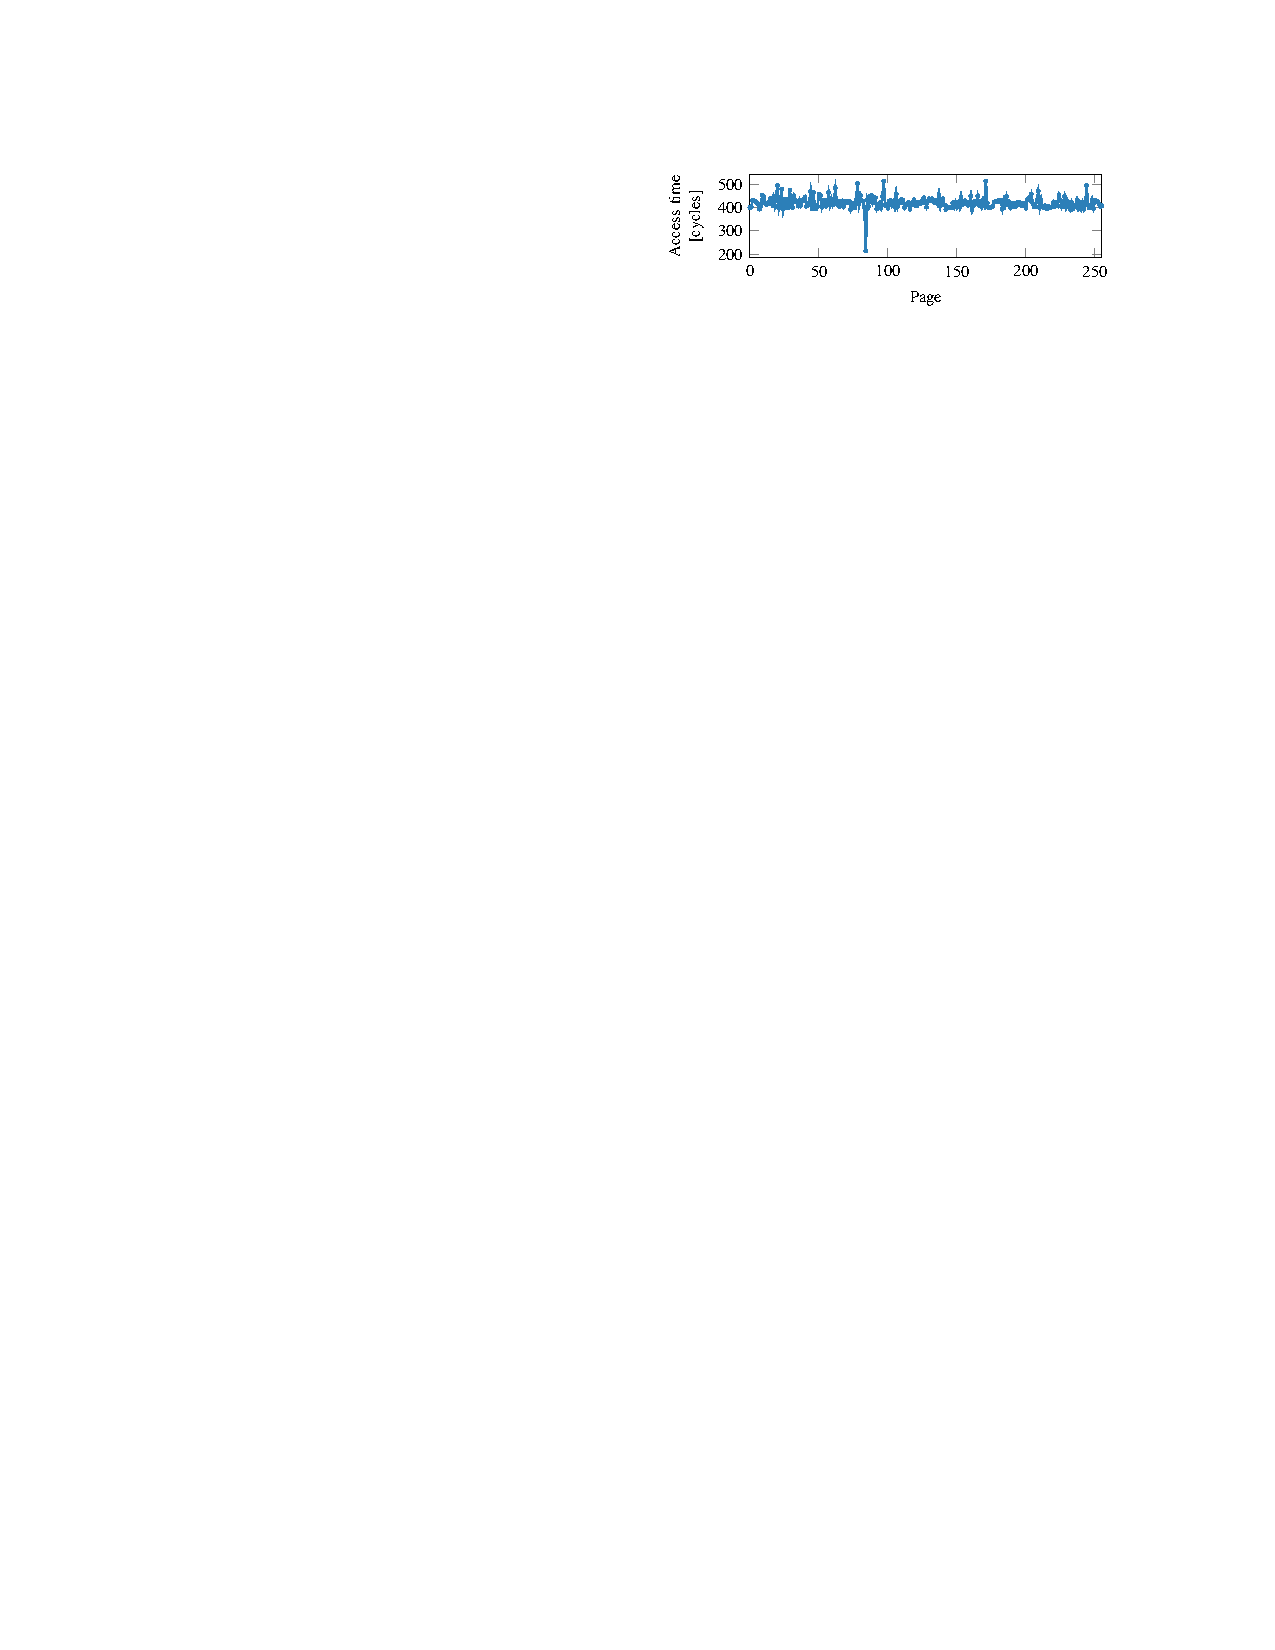
\includegraphics[width=0.75\textwidth]{"img/probe-array.pdf"}
	\caption{Tempo di accesso alle 256 pagine del probe-array. Il grafico mostra una \emph{cache hit} sulla pagina acceduta nel passo~2.~\cite{lipp:meltdown}} % TODO
	\label{fig:probe-array}
\end{figure}


\subsection{Conclusioni}

\begin{lstlisting}[
		language={[x64]Assembler}, float, frame=single,
		numbers=left, numbersep=7pt,
		caption=La sequenza di istruzioni alla base di Meltdown,
		label=lst:meltdown,
		xleftmargin=18.5pt,
		xrightmargin=-18.5pt,
		framexleftmargin=13pt,
		framexrightmargin=-20.5pt
	]
# rcx = indirizzo di memoria kernel
# rbx = probe array
movb (%rcx), %al         # Lettura del segreto
shl  $12, %rax           # Traslazione dell'offset
movq (%rbx, %rax), %rbx  # Trasmissione del segreto
\end{lstlisting}

Il codice presente nel listato \ref{lst:meltdown} mostra in Assembly x86-64

%%

Come abbiamo detto nel paragrafo \ref{sec:spazi-di-indirizzamento}, l'intera memoria fisica viene mappata all'interno dello spazio di indirizzamento del kernel attraversa la cosiddetta \emph{finestra di memoria fisica} \cite{lettieri:paginazione-complementi}.
Essendo la finestra di memoria fisica parte della memoria kernel, dunque, l'attacco Meltdown è in grado non solo di leggere la memoria del kernel, ma anche leggere l'intera memoria fisica, compresi gli spazi virtuali degli altri processi.


